\documentclass[12pt,a4paper]{jsarticle}
\usepackage[dvipdfmx]{graphicx}
\usepackage[dvipdfmx]{color}
\usepackage{listings}
% to use japanese correctly, install jlistings.
\lstset{
  basicstyle={\small\ttfamily},
  identifierstyle={\small},
  commentstyle={\small\itshape\color{red}},
  keywordstyle={\small\bfseries\color{cyan}},
  ndkeywordstyle={\small},
  stringstyle={\small\color{blue}},
  frame={tb},
  breaklines=true,
  numbers=left,
  numberstyle={\scriptsize},
  stepnumber=1,
  numbersep=1zw,
  xrightmargin=0zw,
  xleftmargin=3zw,
  lineskip=-0.5ex
}
\lstdefinestyle{customCsh}{
  language={csh},
  numbers=none,
}
\lstdefinestyle{customRuby}{
  language={ruby},
  numbers=left,
}
\lstdefinestyle{customTex}{
  language={tex},
  numbers=none,
}
\lstdefinestyle{customJava}{
  language={java},
  numbers=left,
}
\begin{document}
\title{卒業論文\\
\vspace{4cm} ユーザメモとwikiを連携するシステムの開発}
\author{ 関西学院大学 理工学部 情報科学科\\\\3550 江本 沙紀}
\date{\vspace{3cm} 2017年  3月\\
\vspace{3cm} 指導教員  西谷 滋人 教授}
\maketitle
\setcounter{tocdepth}{2}
\tableofcontents

\section{開発の背景}
近年,ナレッジマネジメントが企業経営の重要な要素と言われ,導入する企業が増えている.
ナレッジマネジメントとは,個人の持つ知識や情報を組織全体で共有し,
有効に活用することで業績を上げようという経営手法である.
日本語では,「知識管理」などと訳され,「KM」と略されることもある\cite{a}.

ナレッジマネジメントでは,グループ開発において共有する知識は
暗黙知と形式知に分けられる\cite{b}.
暗黙知は主に口伝によって一対一でつたえられたり,あるいは体で覚えるというのが一般的である.
しかし,定着するまでの間は一般的にメモという形で個人的な知識として扱われるのが普通である.
一方で図書館やwebなどでは文書やhyper textとして誰もが読める形で保管,提供される知識は形式知と呼ばれる.

\begin{figure}[htbp]
\begin{center}
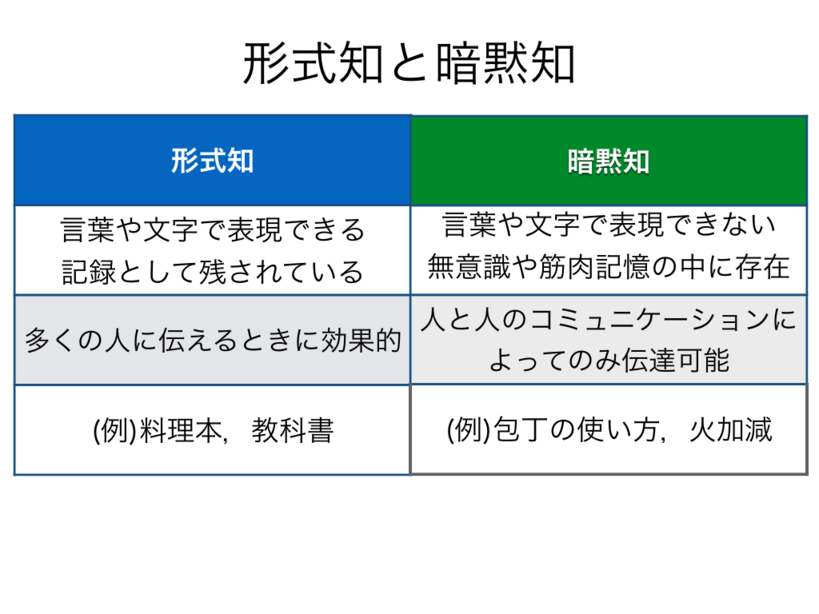
\includegraphics[width=6cm,bb=100 100 600 700]{my_help2hiki_saki.001.png}
\caption{暗黙知と形式知}
\label{default}\end{center}\end{figure}


暗黙知の形式知化はいくつも行われており,google検索したときによく見るQiita.comなどもそれらをまとめるサイトを提供している.
西谷研究室では,各所属学生の暗黙知を形式化するために,my\_helpというgemを開発し,自分のためのメモを残して活用している.
本研究では,西谷研究室内でのナレッジマネジメントを推進するため,
メモソフトmy\_helpからwiki cloneのhikiへ自動変換するシステムの開発と,
my\_helpをよりよいソフトにするためにFrontPageの設計をする.

\begin{figure}[htbp]
\begin{center}
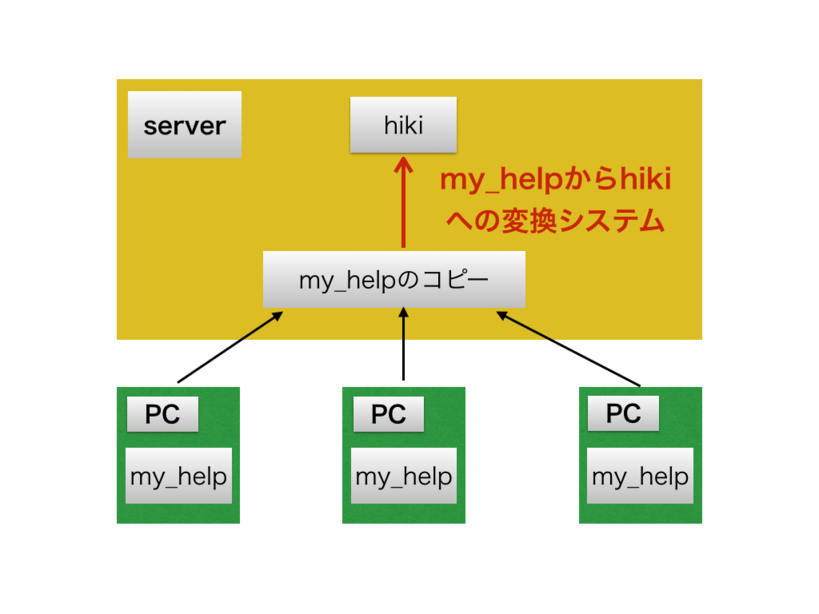
\includegraphics[width=6cm,bb=100 100 600 700]{my_help2hiki_saki.011.png}
\caption{}
\label{default}\end{center}\end{figure}

本論文の構成は次の通りである.
対象とするソフトはあまり一般に普及しているものではないため,
最初にソフトの特徴と簡単な振る舞いを紹介する.
次に3章では作成したソフトの振る舞いとコードの中身を詳述する.
4章では今後これらの変換ソフトを使ってwebを作成するために
プロトタイプを作成し,そこで必要とされる機能について検討を行っている.
最終章では結論をまとめた.


\section{関連するソフトの振る舞い}
本章では,対象とするソフトはあまり一般に普及しているものではないため,
最初にソフト(my\_helpおよびhiki)の特徴と簡単な振る舞いを紹介する.

\subsection{my\_help}
my\_helpは西谷研究室で使用しているユーザ独自のメモを作成するgemである.

gemは正式名称をRubyGemsといい,
Ruby用のライブラリを使う時に必要となるソフトウェアのこと\cite{c}.
パッケージ管理ツールgemがあることで,Ruby用ライブラリの
インストール,アンインストール,バージョン管理などを簡単に
行うことができる.
プログラミング言語Rubyのファイルに付属されていて,
無料で利用することができる.

gemの利点は次の通りである。
\begin{itemize}
\item 標準化された構造があるので,初めてみた人でも分かるようになっている.
\item gemがあることで,簡単にRuby用ライブラリをインストールでき,初心者でもアプリ機能を装備できる.
\item 誰でも作成,配布が可能である.
\end{itemize}

my\_helpが提供するコマンドとその振る舞いをhelp表示から示す.
\begin{quote}\begin{verbatim}
Usage: my_help [options]
    -v, --version                    show program Version.
    -l, --list                       list specific helps
    -e, --edit NAME                  edit NAME help(eg test_help)
    -i, --init NAME                  initialize NAME help(eg test_help).
    -m, --make                       make executables for all helps.
    -c, --clean                      clean up exe dir.
        --install_local              install local after edit helps
        --delete NAME                delete NAME help
        --hiki                       my_help2hiki
\end{verbatim}\end{quote}
my\_helpではhelpの要素をこのhelp表示と同じ構造,項目と対応する記述で表示される.
それぞれの項目はまとまりをつくり,それを-lでリスト表示される.
--versionおよび--listはgem標準に準拠するために用意されている.

my\_helpを研究室内で利用する利点は次の通りである.
\begin{itemize}
\item 研究室内でのメモの書き方が統一できる.
\item どこにメモをしたか忘れることがない.
\item 普段研究の為に使うターミナルから離れること無くメモを残すことができるので,書きたいときにすぐに書くことができる.
\end{itemize}

\subsection{hiki}
Rubyで書かれた高機能・高速Wikiクローン\cite{d}.
CGI(Commond Gateway Interface)を利用して,Webサーバと連動して動く\cite{e}.
西谷研究室では,hikiの形式を利用してサイトを作り,
研究室内での情報共有やgemの使い方などを掲載して閲覧できるようにしている.
また,卒業論文の作成にもhikiの形式で作成している.


\section{方法}
本研究で開発したmy\_helpからhikiへの自動変換ソフトmy\_help2hiki
はmy\_helpのgemに組み込んでいる.
本章では,my\_help2hikiのコマンドとコマンドによる振る舞いを記述する.

\begin{figure}[htbp]\begin{center}
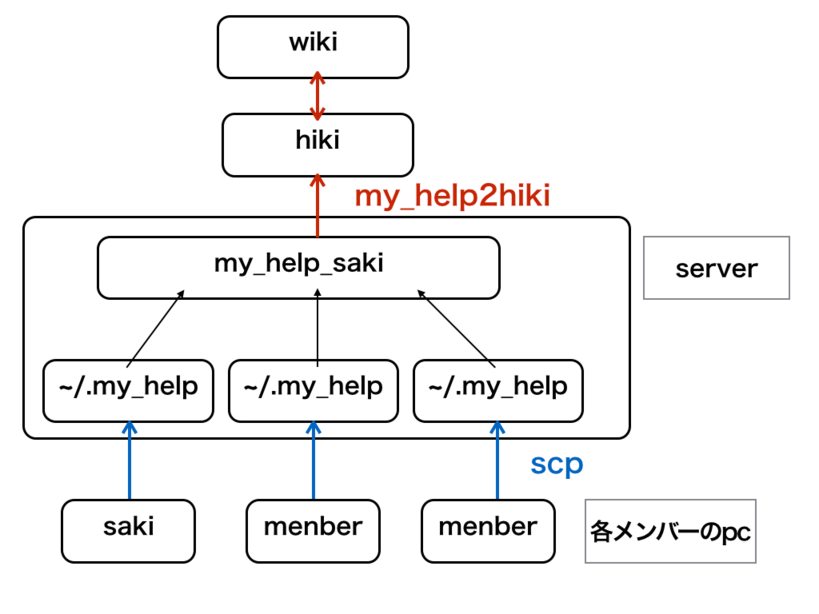
\includegraphics[width=6cm,bb=100 100 600 700]{my_help2hiki_saki.010.png}
\caption{my\_help2hiki}
\label{default}\end{center}\end{figure}

\begin{description}
\item my
my\_help2hikiは図のようになっている,
各学生がmy\_helpで作ったメモは.my\_helpのディレクトリに保存される.
これをscpコマンドを利用してserverのmy\_help\_sakiのディレクトリにコピーする.
コピーしたmy\_helpの内容をmy\_help2hikiを利用してhikiに変換し,wikiで表示する.
\end{description}

\subsection{my\_help/lib/specific\_help.rb}
\begin{description}
\item specific\_help.rbは以下のようになっている
\end{description}
\begin{quote}\begin{verbatim}
/Users/saki/my_help/lib% cat specific_help.rb
# -*- coding: utf-8 -*-
require "optparse"
require "yaml"
require "my_help/version"
require 'fileutils'
require "coderay"

module SpecificHelp
  class Command

    def self.run(file,argv=[])
      new(file, argv).execute
    end

    def initialize(file,argv=[])
      @source_file = file
      @help_cont = YAML.load(File.read(file))
      @help_cont[:head].each{|line| print line.chomp+"\n" } if @help_cont[:head] != nil
      @help_cont[:license].each{|line| print "#{line.chomp}\n" } if @help_cont[:license] != nil
      @argv = argv
    end

    def execute
      if @argv.size==0
        if @source_file.include?('todo')
          @argv << '--all'
        else
          @argv << '--help'
        end
      end
      command_parser = OptionParser.new do |opt|
        opt.on('-v', '--version','show program Version.') { |v|
          opt.version = MyHelp::VERSION
          puts opt.ver
        }
        @help_cont.each_pair{|key,val|
          next if key==:head or key==:license
          opts = val[:opts]
          opt.on(opts[:short],opts[:long],opts[:desc]) {disp_help(key)}
        }
        opt.on('--edit','edit help contents'){edit_help}
        opt.on('--to_hiki','convert to hikidoc format'){to_hiki}
        opt.on('--all','display all helps'){all_help}
        opt.on('--store [item]','store [item] in backfile'){|item| store(item)}
        opt.on('--push', 'push my_todo on remote host'){push}
        opt.on('--remove [item]','remove [item] and store in backfile'){|item| remove(item) }
        opt.on('--add [item]','add new [item]'){|item| add(item) }
        opt.on('--backup_list [val]','show last [val] backup list'){|val| backup_list(val)}
      end
      begin
        command_parser.parse!(@argv)
      rescue=> eval
        p eval
      end
      exit
    end

    def backup_list(val)
      val = val || 10
      print "\n ...showing last #{val} stored items in backup.\n"
      backup=mk_backup_file(@source_file)
      File.open(backup,'r'){|file|
        backup_cont = YAML.load(File.read(backup))
        backup_size = backup_cont.size
        backup_size = backup_size>val.to_i ? val.to_i : backup_size
        backup_keys = backup_cont.keys
        backup_keys.reverse.each_with_index{|item,i|
          break if i>=backup_size
          line = item.to_s.split('_')
          printf("%10s : %8s%8s\n",line[0],line[1],line[2])
        }
      }
    end

    def mk_backup_file(file)
      path = File.dirname(file)
      base = File.basename(file)
      backup= File.join(path,"."+base)
      FileUtils.touch(backup) unless File.exists?(backup)
      return backup
    end

    def store(item)
      if item==nil
        print "spcify --store [item].\n"
        exit
      else
        print "Trying to store #{item}\n"
      end
      backup=mk_backup_file(@source_file)
      unless store_item = @help_cont[item.to_sym] then
        print "No #{item} in this help.  The items are following...\n"
        keys = @help_cont.keys
        keys.each{|key|
          p key
        }
        exit
      end
      p store_name = item+"_"+Time.now.strftime("%Y%m%d_%H%M%S")
      backup_cont=YAML.load(File.read(backup)) || {}
      backup_cont[store_name.to_sym]=store_item
      File.open(backup,'w'){|file| file.print(YAML.dump(backup_cont))}
    end


    def push
      p "push my_todo"
      data_dir = File.join(ENV['HOME'],'.my_help')
      FileUtils.cd(data_dir)
      system "pwd"
      system "rm -rf ~/.my_help/*.yml~"
      system "scp -r ~/.my_help saki@nishitani0:~"
      system "ssh saki@nishitani0 ls ~/.my_help" 


    end


    def add(item='new_item')
      print "Trying to add #{item}\n"
      new_item={:opts=>{:short=>'-'+item[0], :long=>'--'+item, :desc=>item},
          :title=>item, :cont=> [item]}
      @help_cont[item.to_sym]=new_item
      File.open(@source_file,'w'){|file| file.print YAML.dump(@help_cont)}    end

    def remove(item)
      print "Trying to remove #{item}\n"
      store(item)
      @help_cont.delete(item.to_sym)
      File.open(@source_file,'w'){|file| file.print YAML.dump(@help_cont)}
    end

    def edit_help
      system("emacs #{@source_file}")
    end

    def to_hiki
      @help_cont.each_pair{|key,val|
        if key==:head or key==:license
          hiki_disp(val)
        else
          hiki_help(key)
        end
      }
    end

    def all_help
      @help_cont.each_pair{|key,val|
        if key==:head or key==:license
          val[0]+=":"
          disp(val)
        else
          disp_help(key)
        end
      }
    end

    def hiki_help(key_word)
      items =@help_cont[key_word]
      puts "\n!!"+items[:title]+"\n"
      hiki_disp(items[:cont])
    end

    def hiki_disp(lines)
      lines.each{|line| puts "*#{line}"}  if lines != nil
    end

    def disp_help(key_word)
      print_separater
      items =@help_cont[key_word]
      puts CodeRay.scan("-#{items[:title]}:", :Taskpaper).term
      disp(items[:cont])
      print_separater
    end

    def disp(lines)
      lines.each{|line| puts CodeRay.scan("+#{line}", :Taskpaper).term}
    end

    def print_separater
      print "---\n"
    end
    
  end
end
\end{verbatim}\end{quote}

\subsection{my\_help/lib/my\_help.rb}
\begin{description}
\item my\_help.rbは以下のようになっている.
\end{description}
\begin{quote}\begin{verbatim}
/Users/saki/my_help/lib% cat my_help.rb
# -*- coding: utf-8 -*-
require "optparse"
require "yaml"
require "fileutils"
require "my_help/version"
require "systemu"

module MyHelp
  class Command

    def self.run(argv=[])
      new(argv).execute
    end

    def initialize(argv=[])
      @argv = argv
      @default_help_dir = File.expand_path("../../lib/daddygongon", __FILE__)
      @local_help_dir = File.join(ENV['HOME'],'.my_help')
      set_help_dir_if_not_exists
    end

    def set_help_dir_if_not_exists
      return if File::exists?(@local_help_dir)
      FileUtils.mkdir_p(@local_help_dir, :verbose=>true)
      Dir.entries(@default_help_dir).each{|file|
        next if file=='template_help.yml'
        file_path=File.join(@local_help_dir,file)
        next if File::exists?(file_path)
        FileUtils.cp((File.join(@default_help_dir,file)),@local_help_dir,:verbose=>true)
      }
    end

    def execute
      @argv << '--help' if @argv.size==0
      command_parser = OptionParser.new do |opt|
        opt.on('-v', '--version','show program Version.') { |v|
          opt.version = MyHelp::VERSION
          puts opt.ver
        }
        opt.on('-l', '--list', 'list specific helps'){list_helps}
        opt.on('-e NAME', '--edit NAME', 'edit NAME help(eg test_help)'){|file| edit_help(file)}
        opt.on('-i NAME', '--init NAME', 'initialize NAME help(eg test_help).'){|file| init_help(file)}
        opt.on('-m', '--make', 'make executables for all helps.'){make_help}
        opt.on('-c', '--clean', 'clean up exe dir.'){clean_exe}
        opt.on('--install_local','install local after edit helps'){install_local}
        opt.on('--delete NAME','delete NAME help'){|file| delete_help(file)}
        opt.on('--hiki','my_help2hiki'){hiki}
      end
      begin
        command_parser.parse!(@argv)
      rescue=> eval
        p eval
      end
      exit
    end

    def delete_help(file)
      del_files=[]
      del_files << File.join(@local_help_dir,file)
       exe_dir=File.join(File.expand_path('../..',@default_help_dir),'exe')
       del_files << File.join(exe_dir,file)
      p del_files << File.join(exe_dir,short_name(file))
      print "Are you sure to delete these files?[yes]"
      if gets.chomp=='yes' then
        del_files.each{|file| FileUtils.rm(file,:verbose=>true)}
      end
    end

    USER_INST_DIR="USER INSTALLATION DIRECTORY:"
    INST_DIR="INSTALLATION DIRECTORY:"
    def install_local
      Dir.chdir(File.expand_path('../..',@default_help_dir))
      p pwd_dir = Dir.pwd
      status, stdout, stderr = systemu "gem env|grep '#{USER_INST_DIR}'"
      if stdout==""
        status, stdout, stderr = systemu "gem env|grep '#{INST_DIR}'"
      end
      p system_inst_dir = stdout.split(': ')[1].chomp
      if pwd_dir == system_inst_dir
        puts "Download my_help from github, and using bundle for edit helps\n"
        puts "Read README in detail.\n"
        exit
      end
      system "git add -A"
      system "git commit -m 'update exe dirs'"
      system "Rake install:local"
    end

    def short_name(file)
      file_name=file.split('_')
      return file_name[0][0]+"_"+file_name[1][0]
    end

    def make_help
      local_help_entries.each{|file|
        exe_cont="#!/usr/bin/env ruby\nrequire 'specific_help'\n"
        exe_cont << "help_file = File.join(ENV['HOME'],'.my_help','#{file}')\n"
        exe_cont << "SpecificHelp::Command.run(help_file, ARGV)\n"
        file = File.basename(file,'.yml')
        [file, short_name(file)].each{|name|
          p target=File.join('exe',name)
          File.open(target,'w'){|file| file.print exe_cont}
          FileUtils.chmod('a+x', target, :verbose => true)
        }
      }
      install_local
    end

    def clean_exe
      local_help_entries.each{|file|
        next if ['emacs_help','e_h','my_help','my_todo'].include?(file)
        file = File.basename(file,'.yml')
        [file, short_name(file)].each{|name|
          p target=File.join('exe',name)
          FileUtils::Verbose.rm(target)
        }
      }
    end

    def init_help(file)
      p target_help=File.join(@local_help_dir,file+'.yml')
      if File::exists?(target_help)
        puts "File exists. rm it first to initialize it."
        exit
      end
      p template = File.join(@default_help_dir,'template_help.yml')
      FileUtils::Verbose.cp(template,target_help)
    end

    def edit_help(file)
      p target_help=File.join(@local_help_dir,file)
      system "emacs #{target_help}.yml"
    end

    def local_help_entries
      entries= []
      Dir.entries(@local_help_dir).each{|file|
        next unless file.include?('_')
        next if file[0]=='#' or file[-1]=='~' or file[0]=='.'
        entries << file
      }
      return entries
    end

    def list_helps
      print "Specific help file:\n"
      local_help_entries.each{|file|
        file_path=File.join(@local_help_dir,file)
        file = File.basename(file,'.yml')
        begin
          help = YAML.load(File.read(file_path))
        rescue=> eval
          p eval
          print "\n YAML load error in #{file}."
          print "  See the line shown above and revise by\n"
          print "  emacs #{file_path}\n"
          exit
        end
        print "  #{file}\t:#{help[:head][0]}\n"
      }
    end

    def hiki
      system "ls ~/.my_help2"
      system "emacs_help --to_hiki > ~/Sites/hiki-1.0/data/text/emacs_help_saki"
      system "my_todo --to_hiki > ~/Sites/hiki-1.0/data/text/my_todo_saki"
      system "ssh_help --to_hiki > ~/Sites/hiki-1.0/data/text/ssh_help_saki"
      system "open -a safari 'http://localhost/~saki/hiki-1.0/?FrontPage'"
    end

  end
end
\end{verbatim}\end{quote}


\subsection{使用法,コマンド}
\begin{itemize}
\item TARGET --push : 作成したメモ(TARGET)をサーバに送る
\end{itemize}  
\begin{itemize}
\item my\_help --hiki : 作成したメモをhiki形式に変換し,wikiで表示できるようにする.
\end{itemize}

\subsection{コマンドの振る舞い}
\paragraph{TARGET --push}

\begin{figure}[htbp]\begin{center}
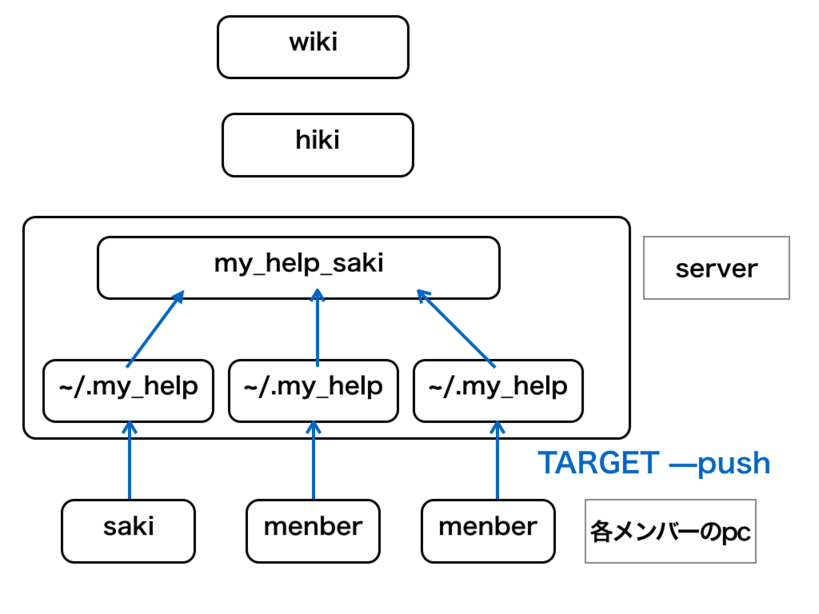
\includegraphics[width=6cm,bb=100 100 600 700]{my_help2hiki_saki.012.png}
\caption{TARGET --push}
\label{default}\end{center}\end{figure}

\begin{quote}\begin{verbatim}
    def push
      p "push my_todo"
      data_dir = File.join(ENV['HOME'],'.my_help')
      FileUtils.cd(data_dir)
      system "pwd"
      system "rm -rf ~/.my_help/*.yml~"
      system "scp -r ~/.my_help saki@nishitani0:~"
      system "ssh saki@nishitani0 ls ~/.my_help" 
\end{verbatim}\end{quote}

\begin{itemize}
\item 3,4行目
\end{itemize}
\begin{description}
\item my\_helpでは,作成したメモが.my\_helpのディレクトリに自動的に追加されるので,
ディレクトリを.my\_helpに移動する.
\end{description}
\begin{itemize}
\item 6行目
\end{itemize}
\begin{description}
\item .my\_helpにメモが追加されるとき,yaml形式のファイルで保存される.
メモを更新すると,一つ前に保存したファイルは*.yml~というファイル名
でバックアップとして残される.
\textbf{rm -rf}で不必要なファイルは削除し,サーバにコピーするときのデータ量を減らしている.
\end{description}

\begin{itemize}
\item 7行目
\end{itemize}
\begin{description}
\item
\textbf{scp -r ~/[directory名] [server名]}
serverにssh接続を行い,directoryをserverにコピーする.
-rはディレクトリ全体をコピーすることを示している.
西谷研究室で利用しているnishitani0というサーバにコピーしている.
\end{description}

\begin{itemize}
\item 8行目
\end{itemize}
\begin{description}
\item nishitani0にssh接続し.my\_helpの中身を書き出して,
コピーができているかコマンドを実行した時に確認が行えるようにしている.
\end{description}

\paragraph{my\_help --hiki}

\begin{figure}[htbp]\begin{center}
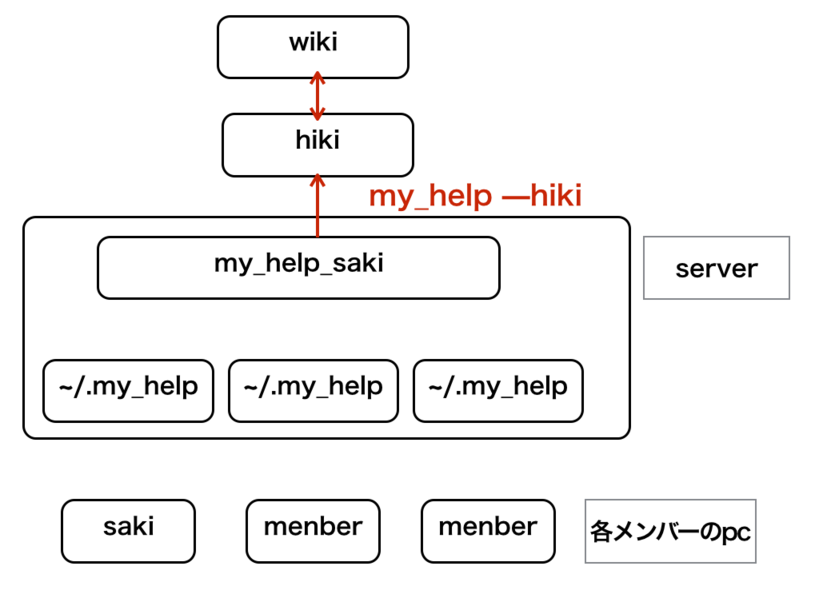
\includegraphics[width=6cm,bb=100 100 600 700]{my_help2hiki_saki.013.png}
\caption{my\_help2hiki}
\label{default}\end{center}\end{figure}


\begin{quote}\begin{verbatim}
def hiki
      p 'my_help2hiki'
      system "emacs_help --to_hiki > ~/Sites/hiki-1.0/data/text/emacs_help_saki"
      system "my_todo --to_hiki > ~/Sites/hiki-1.0/data/text/my_todo_saki"
      system "ssh_help --to_hiki > ~/Sites/hiki-1.0/data/text/ssh_help_saki"
      system "open -a safari 'http://localhost/~saki/hiki-1.0/?FrontPage'"
    end
\end{verbatim}\end{quote}
\begin{itemize}
\item 2-4行目
\end{itemize}
\begin{description}
\item my\_helpには,\textbf{TARGET --to\_hiki}というコマンドがあり,これによって
yaml形式で保存されているメモをhiki形式で書き出すことができる.
この --hiki のコマンドを使ってhiki形式にしたものを,wikiで表示することのできる
フォルダである\textbf{~/Sites/hiki-1.0/data/text/}に入れることで,wikiでの表示を可能にしている.
emacs\_help,my\_todo,ssh\_helpは全て私のmy\_helpに入っているメモ.
\end{description}

\begin{itemize}
\item 5行目
\end{itemize}
\begin{description}
\item wikiのページ図6に示したFrontPageを表示するコマンド.
これによりメモが更新されているのを即時確認することができる.
FrontPageは以下のようになっている.
\end{description}
\begin{quote}\begin{verbatim}
!saki's help
*[[ssh_help_saki]]
*[[my_todo_saki]]
*[[emacs_help_saki]]
\end{verbatim}\end{quote}
\begin{description}
\item 先頭に\textbf{!}をつけることで1行目のsaki's helpを見出しにし,
2~4行目は\textbf{*}によって箇条書き,角括弧でリンクになっている.
\end{description}

\begin{figure}[htbp]\begin{center}
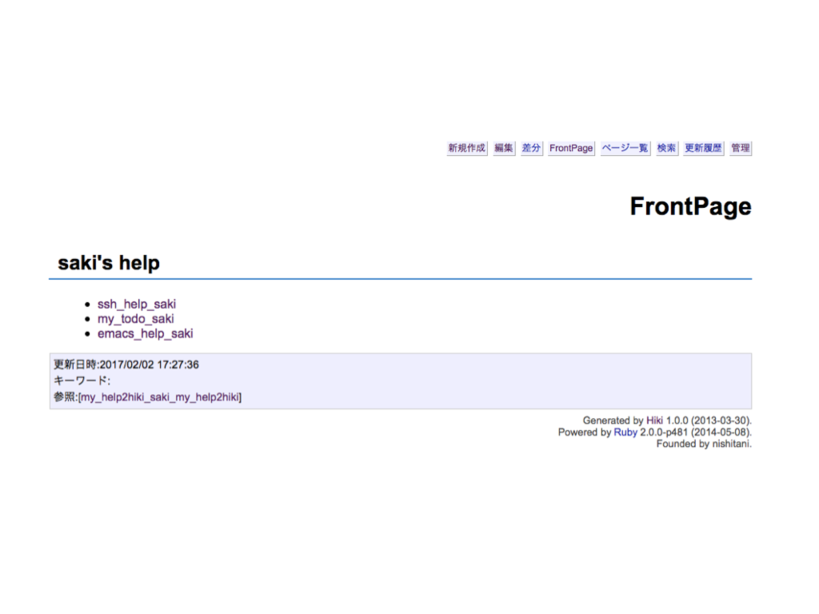
\includegraphics[width=6cm,bb=100 100 600 700]{my_help2hiki_saki.002.png}
\caption{コマンドを実行したときに開くFrontPage }
\label{default}\end{center}\end{figure}


\section{FrontPageの設計}
my\_helpをよりよくするための設計を示す.
各学生のFrontPage,各helpのページに分けて,実装すると便利になる理由と共に記述している.

\begin{figure}[htbp]\begin{center}
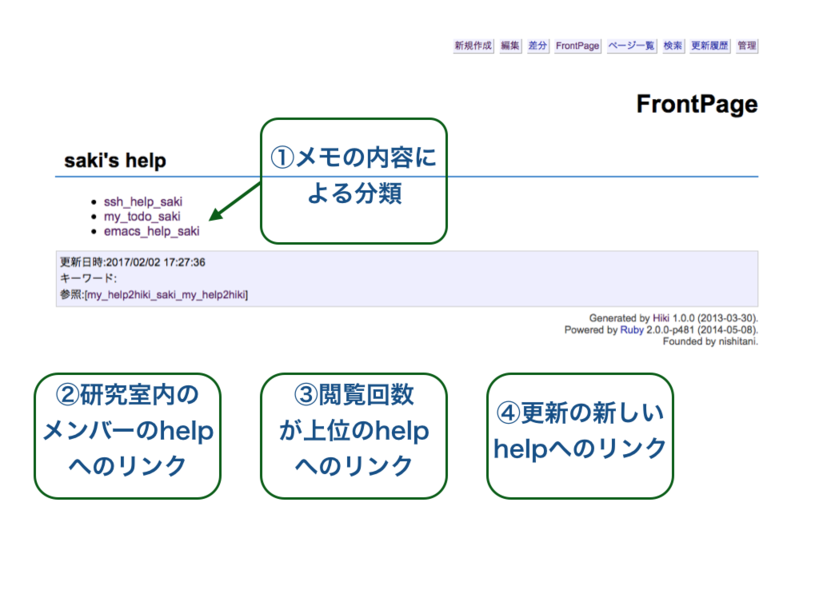
\includegraphics[width=6cm,bb=100 100 600 700]{my_help2hiki_saki.008.png}
\caption{FrontPage}
\label{default}\end{center}\end{figure}

\paragraph{1.メモの内容による分類}
\begin{description}
\item 研究室内の所属学生の利用するハードウェア,ソフトウェアは同じものが多い.
例えば,西谷研究室ではハードウェアは全員がmacを使い,プログラム作成はターミナル,
hiki文書の作成にはmiというソフトを使用している.
それぞれのハードウェア,ソフトウェアに関するhelpを分類分けしておくことで,
調べたいことに関してのhelpを探しやすくすることができる.
\end{description}

\paragraph{2.研究室内のメンバーのhelpへのリンク}
\begin{description}
\item 同研究室の他学生のFrontPageへのリンクを作る.
同回のメンバーが書いたメモを見たい,先輩のメモを見たい,他メンバーの研究を知りたい.
そのときの目的に応じて閲覧するhelpを選ぶことができる.
\end{description}

\paragraph{3.閲覧回数が上位のhelpへのリンク}
\begin{description}
\item 閲覧回数の多い,研究室内の学生が見た回数の多いものへのリンクを作る.
研究室に入ってばかりで分からないことが多いときにこのhelpを見れば,研究室のことが理解できる.
知らなくても支障はないが,知っておくと便利な豆知識を得ることが期待される.
\end{description}

\paragraph{4.更新の新しいhelpへのリンク}
\begin{description}
\item 更新が新しいものを表示しておくことで,メンバーが得た最新の知識を得やすくなる.
また,他メンバーがどのような研究を進めているか,どのようなことを調べてたのかを知ることができ,自分の研究の進め方の参考にすることができる.
\end{description}

\begin{figure}[htbp]\begin{center}
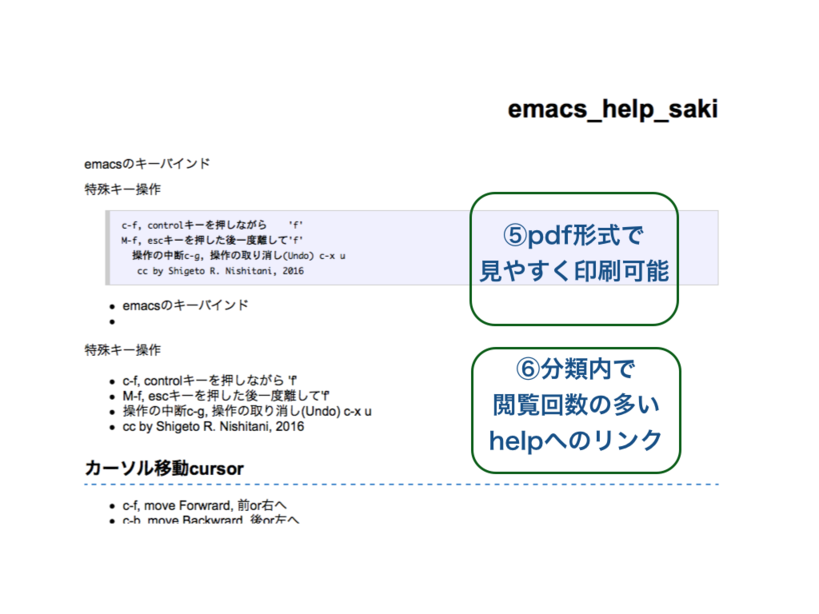
\includegraphics[width=6cm,bb=100 100 600 700]{my_help2hiki_saki.009.png}
\caption{例 emacs\_help}
\label{default}\end{center}\end{figure}

\paragraph{5.pdf形式で見やすく印刷可能}
\begin{description}
\item 紙媒体で持ち歩くことを可能にするために,pdf形式に変換することで見やすくしたhelpを印刷することができる.
emacs\_helpを例にして考える.このhelpはターミナルでemacsを使うときのキーバインドを表している.
ターミナルを利用していると,このhelpを開きながら操作することは手間がかかる.
そこで見やすくしたhelpを紙に印刷することでこの手間を省くことができる.
西谷研究室ではhikiからlatexへの変換ソフト,hiki2latexがあるので,作成可能だと考えられる.
\end{description}

\paragraph{6.分類内で閲覧回数の多いhelpへのリンク}
\begin{description}
\item 分類内で閲覧回数の多いhelpは他メンバーの多くが得た知識なので,
知っておくべき知識であるといえる.
自分がその分類内で分からないことを解決する手がかりになることが期待される
\end{description}


\section{結果}
\begin{quote}\begin{verbatim}
/Users/saki% my_help --list
Specific help file:
  emacs_help	:emacsのキーバインド
  memo_help	:ヘルプのサンプル雛形
  my_todo	:my_todo
  ssh_help	:sshのhelp
\end{verbatim}\end{quote}

これは私のmy\_helpの中身を書き出している.
下がemacs\_helpの中身である.

\begin{quote}\begin{verbatim}
/Users/saki% emacs_help --all
emacsのキーバインド

特殊キー操作
  c-f, controlキーを押しながら    'f'
  M-f, escキーを押した後一度離して'f'
    操作の中断c-g, 操作の取り消し(Undo) c-x u
     cc by Shigeto R. Nishitani, 2016
+emacsのキーバインド:
+
特殊キー操作
+  c-f, controlキーを押しながら    'f'
+  M-f, escキーを押した後一度離して'f'
+    操作の中断c-g, 操作の取り消し(Undo) c-x u
+     cc by Shigeto R. Nishitani, 2016:
---
-カーソル移動cursor:
+c-f, move Forwrard,    前or右へ
+c-b, move Backwrard,   後or左へ
+c-a, go Ahead of line, 行頭へ
+c-e, go End of line,   行末へ
+c-n, move Next line,   次行へ
+c-p, move Previous line, 前行へ
---
---
-ページ移動page:
+c-v, move Vertical,          次のページへ
+M-v, move reversive Vertical,前のページへ
+c-l, centerise Line,       現在行を中心に
+M-<, move Top of file,    ファイルの先頭へ
+M->, move Bottom of file, ファイルの最後尾へ
---
---
-ファイル操作file:
+c-x c-f, Find file, ファイルを開く
+c-x c-s, Save file, ファイルを保存
+c-x c-w, Write file NAME, ファイルを別名で書き込む
---
---
-編集操作edit:
+c-d, Delete char, 一字削除
+c-k, Kill line,   一行抹消,カット
+c-y, Yank,        ペースト
+c-w, Kill region, 領域抹消,カット
+領域選択は,先頭or最後尾でc-spaceした後,最後尾or先頭へカーソル移動
+c-s, forward incremental Search WORD, 前へWORDを検索
+c-r, Reverse incremental search WORD, 後へWORDを検索
+M-x query-replace WORD1 <ret> WORD2:対話的置換(y or nで可否選択)
---
---
-ウィンドウ操作window:
+c-x 2, 2 windows, 二つに分割
+c-x 1, 1 windows, 一つに戻す
+c-x 3, 3rd window sep,縦線分割
+c-x o, Other windows, 次の画面へ移動
---
---
-バッファー操作buffer(すでにopenしてemacsにバッファーされたfile):
+c-x b, show Buffer,   バッファのリスト
+c-x c-b, next Buffer, 次のバッファへ移動
---
---
-終了操作quit:
+c-x c-c, Quit emacs, ファイルを保存して終了
+c-z, suspend emacs,  一時停止,fgで復活
\end{verbatim}\end{quote}

このように各学生のメモを何種類も作成できるが,自分のパソコンでしか見ることができなかった.
本研究によるmy\_help2hikiを使うことで,図6のようにmy\_helpをwikiで表示可能になり,
各学生のメモを研究室内で共有することができるようになる.
さらに4章で述べたような設計ができれば,研究室内のナレッジマネジメントは
今より推進させると考えている.

\section{今後の課題}
西谷研究室には内部サイトがあり,研究室内で使うシステムのマニュアルなどが公開されている.
hiki形式への変換ができればwikiで表示することはできるようになるが,
my\_help2hikiのコマンドでwikiのページを作成しても,現段階では研究室内全員が見ることはできない.
内部サイトへの自動表示を可能にするようなコマンドを作る必要があると考えられる.
今後,作成したmy\_helpの設計に基づき実装を進めてほしい.
\begin{thebibliography}{5}
\bibitem{a}「e-Words ナレッジマネジメント」,{http://e-words.jp/w/ナレッジマネジメント.html},2017/1/27アクセス.
\bibitem{b}ニック・ミルトン,「プロジェクト・ナレッジ・マネジメント」(生産性出版,東京都渋谷区渋谷,2009年発行),pp.4-5.
\bibitem{c}「Ruby on Rails 初心者必見!パッケージ管理ツール『gem』を徹底解説」,{https://blog.codecamp.jp/rails-gem},2017/1/27アクセス.
\bibitem{d}「Hiki -Front Page-」,{http://hikiwiki.org/ja/},2017/1/27アクセス.
\bibitem{e}「Hiki -Wikipedia」,{https://ja.wikipedia.org/wiki/Hiki},2017/1/27アクセス.
\end{thebibliography}
\end{document}